
\section{Emissão de sinais}

    \subsection{Equação do sinal}
    \begin{frame}{Definição de onda}
        \begin{equation*}
            w(x, y, t, \theta, r, \phi, \lambda, \omega) = \frac{\sin\left(\mathcal{aux}\right)+ \cos\left(\mathcal{aux}\right)}{\sqrt{2}}
        \end{equation*}

        \begin{equation*}
            \mathcal{aux}(x, y, t, \theta, r, \phi, \lambda, \omega) =
            \frac{2\pi}{\lambda} \cdot \sqrt{(y - y_0)^2+(x - x_0)^2} + \omega \cdot t + \phi
        \end{equation*}

        \begin{equation*}
            x_0 = r_0 \cdot \cos(\theta)
        \end{equation*}

        \begin{equation*}
            y_0 = r_0 \cdot \sin(\theta)
        \end{equation*}

        \begin{equation*}
            r_0 = r \cdot \lambda
        \end{equation*}

    \end{frame}

    \subsection{Frente de onda}
    \begin{frame}{Emissão de sinal radial}
        % % \begin{center}
\begin{circuitikz}[american, voltage shift=0.5, line width=0.5]
    % Variables
    \def\D{\N*\T}        
    \def\wavelength{1}
    \def\d{0.5*\wavelength}

    
    \begin{axis}[
        at={(0,0)},
        view={0}{90},
        hide axis,
        colormap={custom}{color=(white) color=(Gray)},
        trig format plots=rad,
        x=1cm,
        y=1cm,
        z=0cm,
    ]
    
    \clip[] (-0.5,-4) rectangle (13.1,4);
    \addplot3[
        data cs=polar,
        samples=25,
        domain=0:2*pi,
        domain y=0:15,
        samples y=100,
        surf,shader=interp,
    ] {sin(2*pi*y + 0.5*pi)};



    \coordinate (O) at (0,0);
    % \draw [help lines, dashed] (-5,-3) grid (5,3); % desenha grid
    % \draw [red] (O) node[draw,cross out] {}; % marca pont(0,0) 

    \draw[thick]
        (0,0) node[dinantenna]{}
    ;
        



    \end{axis}
        

\end{circuitikz}
% \end{center}
        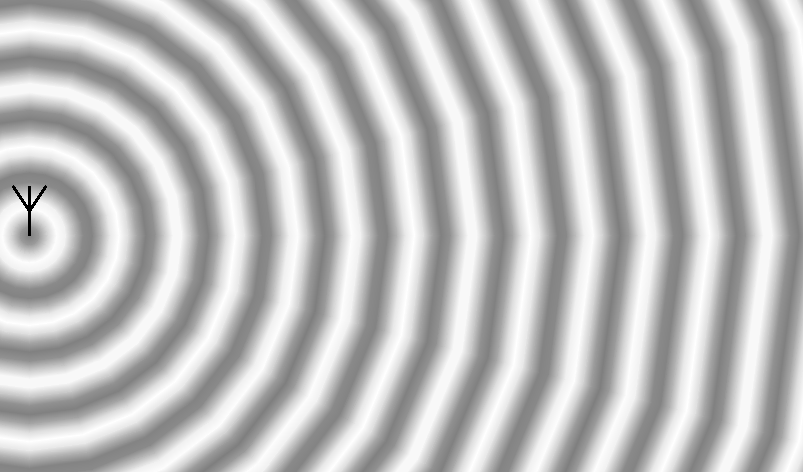
\includegraphics{../pictures/signal.pdf}
    \end{frame}

    \begin{frame}{Frentes de onda}
        % \begin{circuitikz}[american, voltage shift=0.5, line width=0.5]
    % Variables
    \def\T{1}
    \def\A{1}
    \def\N{5}
    \def\D{\N*\T}
    \def\wavelength{1}
    \def\d{0.5*\wavelength}


    \begin{axis}[
        at={(0,0)},
        view={0}{90},
        hide axis,
        colormap={custom}{color=(white) color=(Gray)},
        trig format plots=rad,
        x=1cm,
        y=1cm,
        z=0cm,
    ]
    \clip[] (-0.5,-4) rectangle (13.1,4);
    \addplot3[
        data cs=polar,
        samples=25,
        domain=0:2*pi,
        domain y=0:15,
        samples y=100,
        surf,shader=interp,
    ] {sin(2*pi*y/\wavelength + 0.5*pi)};



        \coordinate (O) at (0,0);
        % \draw [help lines, dashed] (-5,-3) grid (5,3); % desenha grid
        % \draw [red] (O) node[draw,cross out] {}; % marca pont(0,0)

        \draw[thick]
            (0,0) node[dinantenna]{}
        ;

        % \clip[] (-0.1,-4) rectangle (13.1,4);
        \pgfplotsinvokeforeach{1,2,...,13} {
        \draw [Black] (axis cs:0,0) circle (#1*\wavelength);
        }


    \end{axis}


\end{circuitikz}
        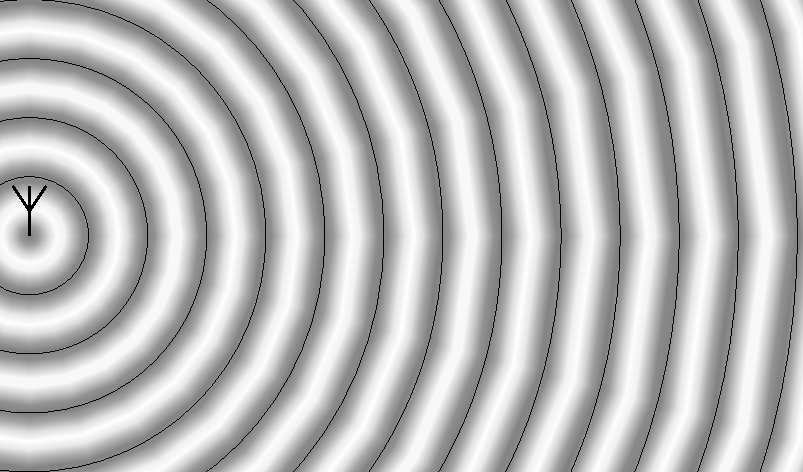
\includegraphics{../pictures/signal+lines.pdf}
    \end{frame}

    \begin{frame}{Representação de frentes de onda}
            \begin{circuitikz}[american, voltage shift=0.5, line width=0.5]

        \def\wavelength{1}
        \def\d{0.5*\wavelength}

        \coordinate (O) at (0,0);
        \coordinate (antenna) at (0,0);
        % \draw [help lines, dashed] (-5,-3) grid (5,3); % desenha grid
        % \draw [red] (O) node[draw,cross out] {}; % marca pont(0,0) 

        \draw[thick]
            (antenna) node[dinantenna]{}
        ;
        
        \clip[] (-0.5,-4) rectangle (13.1,4);
        \draw [gray, thin]
        \foreach \x in {1,2,...,13} {
            (antenna) circle (\x*\wavelength)
        }
        ;

        % \foreach \x in {0,60,...,300} {
        %     \draw[thick] (\x:1 cm) -- (\x + 60:1 cm);
            
        %     \draw (\x + 30:1.732 cm) node[Gray, circ]{};
        %     \draw[Gray, dashed] (\x:1 cm) -- ++(\x: 0.9cm);
        %     \draw[Gray, dotted]
        %     %     % (\x:1 cm) arc (\x+240:\x+180:1cm)
        %         (\x:1 cm) arc [start angle=\x+120, delta angle=110, radius=1cm]
        %         (\x:1 cm) arc [start angle=\x+120, delta angle=-50, radius=1cm]
        %     ;
        % }
    
        % \draw (0,0) node [circ] {} node [below left,font={\scriptsize\bfseries}] {BS};
        % \draw[thick, densely dotted] (0,0) circle (1cm);
        
        % \draw[-latex] (0,0) -- (0:1cm) node[midway, below] {$R_c$};
        % \draw[-latex] (0,0) -- (90:0.866cm) node[midway, left] {$R$};
            
    \end{circuitikz}

    \end{frame}

\subsection{Onda plana}

    \begin{frame}{Comportamento da onda no espaço próximo}
            % \resizebox{\textwidth}{!}{%
    \begin{circuitikz}[american, voltage shift=0.5, line width=0.5]

        \def\wavelength{0.5}
        \def\d{0.5*\wavelength}

        \def\closeRange{1}
        \def\farRange{\closeRange+30}

        \coordinate (O) at (0,0);
        \coordinate (antenna) at (-\closeRange,0);
        % \draw [help lines, dashed] (-5,-3) grid (5,3); % desenha grid
        % \draw [red] (O) node[draw,cross out] {}; % marca pont(0,0)

        \draw[thick]
            (antenna) node[dinantenna, scale=0.75]{}
        ;

        % \draw (\closeRange-0.5,-4) rectangle (\farRange+0.1,4);
        \clip (-0.75,-1.5) rectangle (12.1,1.5);
        \foreach \x [evaluate={\z=int((\x+\closeRange));}] in {0,...,30} {
            \draw [gray, thin, opacity=0.5] (antenna) circle (\z*\wavelength);
            \draw [black]
            (antenna) ++ (\z*\wavelength,0)
            node[anchor=south, font = {\footnotesize\bfseries}, rotate=-90,scale=0.75]{$\z\lambda$}
            ++(0, -4)
            -- ++(0,8);
        }

        \draw [Red, thick] (antenna) ++ (8*\wavelength,-4) -- ++(0,8);

        % \foreach \x in {0,60,...,300} {
        %     \draw[thick] (\x:1 cm) -- (\x + 60:1 cm);

        %     \draw (\x + 30:1.732 cm) node[Gray, circ]{};
        %     \draw[Gray, dashed] (\x:1 cm) -- ++(\x: 0.9cm);
        %     \draw[Gray, dotted]
        %     %     % (\x:1 cm) arc (\x+240:\x+180:1cm)
        %         (\x:1 cm) arc [start angle=\x+120, delta angle=110, radius=1cm]
        %         (\x:1 cm) arc [start angle=\x+120, delta angle=-50, radius=1cm]
        %     ;
        % }

        % \draw (0,0) node [circ] {} node [below left,font={\scriptsize\bfseries}] {BS};
        % \draw[thick, densely dotted] (0,0) circle (1cm);

        % \draw[-latex] (0,0) -- (0:1cm) node[midway, below] {$R_c$};
        % \draw[-latex] (0,0) -- (90:0.866cm) node[midway, left] {$R$};

    \end{circuitikz}
  % }

    \end{frame}

    \begin{frame}{Comportamento da onda em espaço distante (\textit{far field})}
        \resizebox{\textwidth}{!}{%
    \begin{circuitikz}[american, voltage shift=0.5, line width=0.5]

        \def\wavelength{0.75}
        \def\d{0.5*\wavelength}

        \def\closeRange{25}
        \def\farRange{\closeRange+20}

        \coordinate (O) at (0,0);
        \coordinate (antenna) at (-\closeRange*\wavelength,0);
        % \draw [help lines, dashed] (-5,-3) grid (5,3); % desenha grid
        % \draw [red] (O) node[draw,cross out] {}; % marca pont(0,0) 

        % \draw[thick]
        %     (antenna) node[dinantenna]{}
        % ;
        
        % \draw (-0.5,-1.5) rectangle (13.1,1.5);
        \clip (-0.5,-1.5) rectangle (13.1,1.5);
        \foreach \x [evaluate={\z=int((\x+\closeRange));}] in {0,...,20} {
            \draw [black, thick] 
            (antenna) ++ (\z*\wavelength,0) 
            node[anchor=south, font = {\footnotesize\bfseries}, rotate=-90]{$\z\lambda$}
            ++(0, -4) 
            -- ++(0,8);
            \draw [gray, thin] (antenna) circle (\z*\wavelength);
        }


        % \foreach \x in {0,60,...,300} {
        %     \draw[thick] (\x:1 cm) -- (\x + 60:1 cm);
            
        %     \draw (\x + 30:1.732 cm) node[Gray, circ]{};
        %     \draw[Gray, dashed] (\x:1 cm) -- ++(\x: 0.9cm);
        %     \draw[Gray, dotted]
        %     %     % (\x:1 cm) arc (\x+240:\x+180:1cm)
        %         (\x:1 cm) arc [start angle=\x+120, delta angle=110, radius=1cm]
        %         (\x:1 cm) arc [start angle=\x+120, delta angle=-50, radius=1cm]
        %     ;
        % }
    
        % \draw (0,0) node [circ] {} node [below left,font={\scriptsize\bfseries}] {BS};
        % \draw[thick, densely dotted] (0,0) circle (1cm);
        
        % \draw[-latex] (0,0) -- (0:1cm) node[midway, below] {$R_c$};
        % \draw[-latex] (0,0) -- (90:0.866cm) node[midway, left] {$R$};
            
    \end{circuitikz}
}



% \begin{center}
%     % \resizebox{\textwidth}{!}{%
%     \begin{circuitikz}[american, voltage shift=0.5, line width=0.5]

%         \def\wavelength{1}
%         \def\d{0.5*\wavelength}

        
%         \def\closeRange{-50}
%         \def\closeRangePlus{\closeRange+1}
%         \def\farRange{\closeRange+13}

%         \coordinate (O) at (0,0);
%         \coordinate (antenna) at (\closeRange,0);
%         % \draw [help lines, dashed] (-5,-3) grid (5,3); % desenha grid
%         % \draw [red] (O) node[draw,cross out] {}; % marca pont(0,0) 

%         % \draw[thick]
%         %     (antenna) node[dinantenna]{}
%         % ;
        
%         % \draw (\closeRange-0.5,-4) rectangle (\farRange+0.1,4);
%         \clip (-0.5,-4) rectangle (13.1,4);
%         \foreach \x in {0,...,13} {
%         \draw [black, thick] (antenna) ++ ({(\x-\closeRange)*\wavelength}, -4) -- ++(0,8);
%         \draw [gray, thin] (antenna) circle ({(\x-\closeRange)*\wavelength});
%         }

%         % \foreach \x in {0,60,...,300} {
%         %     \draw[thick] (\x:1 cm) -- (\x + 60:1 cm);
            
%         %     \draw (\x + 30:1.732 cm) node[Gray, circ]{};
%         %     \draw[Gray, dashed] (\x:1 cm) -- ++(\x: 0.9cm);
%         %     \draw[Gray, dotted]
%         %     %     % (\x:1 cm) arc (\x+240:\x+180:1cm)
%         %         (\x:1 cm) arc [start angle=\x+120, delta angle=110, radius=1cm]
%         %         (\x:1 cm) arc [start angle=\x+120, delta angle=-50, radius=1cm]
%         %     ;
%         % }
    
%         % \draw (0,0) node [circ] {} node [below left,font={\scriptsize\bfseries}] {BS};
%         % \draw[thick, densely dotted] (0,0) circle (1cm);
        
%         % \draw[-latex] (0,0) -- (0:1cm) node[midway, below] {$R_c$};
%         % \draw[-latex] (0,0) -- (90:0.866cm) node[midway, left] {$R$};
            
%     \end{circuitikz}
%   % }
% \end{center}

    \end{frame}
